\documentclass{article}

% ------ TEMPLATE ------ %

% ---------------------- %

% ------ PACKAGES ------ %

\usepackage{charter}
\usepackage{geometry}
\usepackage{amsmath}
\usepackage{amssymb}
\usepackage{float}
\usepackage{graphicx}
\usepackage{tabularx}
\usepackage{array}
\usepackage{subcaption}
\usepackage{enumitem}
\usepackage{titlesec}
\usepackage{hyperref}
\usepackage{xcolor}
\usepackage{pifont}
\usepackage{fancyvrb}
\usepackage{listings}
\usepackage{multirow}
\usepackage{ulem}
\usepackage{minted}

% ---------------------- %

% ------ GENERALS ------ %

\setlist[itemize]{label=\scriptsize\textbullet}
\setlist[itemize]{noitemsep, topsep=1pt}
\setlist[enumerate]{noitemsep, topsep=1pt}

\titleformat{\chapter}[hang]
{\normalfont\huge\bfseries}{\thechapter}{1em}{}
\titleformat{\subsubsection}{\large\bfseries}{\thesubsubsection}{1em}{}

% ---------------------- %

% ------- COLORS ------- %

\hypersetup{
    colorlinks=true,
    linkcolor=blue!50!black,
    urlcolor=blue,
    citecolor=blue,
    pdfborder={0 0 0}
}

% ---------------------- %

% ------ COMMANDS ------ %

\newcommand{\vmark}{\textcolor{teal}{\ding{51}}}
\newcommand{\xmark}{\textcolor{red!70!black}{\ding{55}}}
\newcommand{\newpar}[0]{\vspace{2mm}\noindent}
\newcommand{\htitle}[1]{\newpar\textbf{#1 -}}
\newcommand{\ititle}[1]{\newpar\hspace{1em}\textbf{#1}}
\newcommand{\hyperlabel}[1]{\hypertarget{#1}\phantomsection\label{#1}}
\newcommand{\hyperitem}[2]{\item \hyperlink{#1}{#2}\leaders\hbox to 0.8em{\hss.\hss}\hfill\hbox to 1.8em{\hss\pageref{#1}}}
\newcommand{\stdtilde}[0]{\raise.17ex\hbox{$\scriptstyle\sim$}}
\newcommand{\xor}[0]{\char`\^}
\newcommand{\saveformula}[2]{\newbox{#1}\savebox{#1}{#2}}
\newcommand{\useformula}[1]{\usebox{#1}}

% ---------------------- %

\begin{document}

% -------- HEAD -------- %

\pagenumbering{gobble}

\begin{center}

	\fontsize{20pt}{30pt}\selectfont
	Well MEing

	\vspace{2cm}

	\fontsize{25pt}{45pt}\selectfont
	\textbf{Developer Guide}

	\vfill

	\fontsize{12pt}{18pt}\selectfont
	Matteo Bettiati \\
	Lorenzo Bianchi \\
	Alessio Caggiano \\
	Francesco Ostidich \\
	Denis Sanduleanu \\

	\vspace{1cm}

	\today \\
	\vspace{12pt}
	Version: 0.1
	\normalsize

\end{center}

\newpage
\pagenumbering{arabic}
\tableofcontents
\newpage

% ---------------------- %

% -------- BODY -------- %

\section{Introduction}

This document provides a low level description of the system architecture, outlining the deployment structure, code organization, and exposed endpoints.
It also showcases the strategies an techniques chosen for designing the AI modules.

The goal is to ensure maintainability, scalability, and clarity for future development.
Finally, contributions from each team member are summarized.

\section{Deployment view}

The system follows a cloud-based, serverless architecture, with the frontend on mobile platforms, and functionalities hosted on Firebase.

The client is a Swift-based iOS application running on iPhones, responsible for the user interface and local interactions.

All backend services are hosted on Firebase, leveraging its functions, written in Python, to handle endpoints and AI-related processing.
Firebase Authentication manages user login and access control, while a NoSQL realtime database allow for storing and retrieving application data.
For AI capabilities, the backend integrates with Google Cloud's Vertex AI and Generative AI services to handle inference and model execution tasks.

\begin{figure}[H]
	\centering
	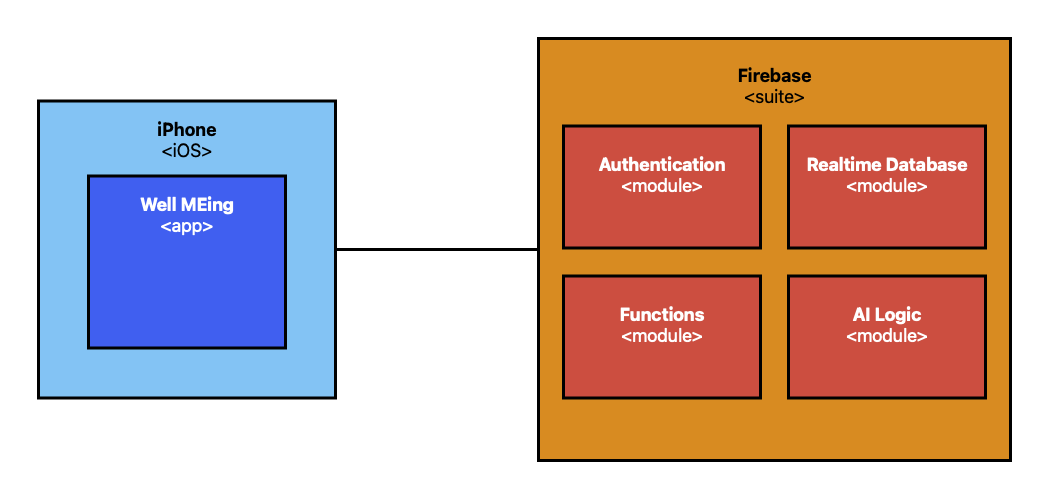
\includegraphics[width=0.6\textwidth]{images/deployment-view.png}
\end{figure}

\section{Code structure}

The following sections describe the project folder trees for both the client Swift app and the Firebase Python functions (with focus on the hosted code for running the AI).

\subsection{Client}

\begin{verbatim}
Well-MEing/
  - Models/
  - Services/
  - Views/
      - Branded/
      - Contents/
      - Elements/
      - InputSelectors/
      - InputTypes/
      - Sections/
\end{verbatim}

The client project contains a little "Models" folder in which the main objects used throughout the client codebase are defined.
These resembles either DB entities or DTOs, which, in general, coincide.
The main model class is the \verb|UserCache|, which defines a shared static object that is the entrypoint for reaching all user's fetched information, like habits, reports, or personal data.

The "Services" folder mainly contains the code used to express the logic executing on the client.
In particular, here is found the code for enabling authentication, making requests to the backend, processing past data, enabling the text-to-speech recognition, and importing data from Apple Health.

Finally, the "View" folder, being the client a frontend application, contains all the SwiftUI structs which compose the presentation layer.
Subfolders helps to organize view components based on their purposes.
The three main app sections are defined in the "Sections" folder.
The other main pages that are placed above the navigation stack base are found in the "Contents" folder.
General little components are found in the "Elements" folder, whereas others that are more theme-related are found in the "Branded" one.
The metric input formats may have slightly different definitions, as they can be used either as simple type previews in the habit creation panel, or as concrete selectors for the habit logging; they are thus organized separately in two dedicated folders.

\subsection{Server}

\section{Endpoints}

\section{AI Design}

\section{Contributions}

\end{document}
